\documentclass[a4paper,12pt]{extarticle}


%% Language and font encodings
\usepackage[english]{babel}
\usepackage[utf8x]{inputenc}
\usepackage[T1]{fontenc}

%% Sets page size and margins
\usepackage[a4paper,top=3cm,bottom=3cm,left=3cm,right=3cm,marginparwidth=2.5cm]{geometry}

%% Useful packages
\usepackage{amsmath}
\usepackage{graphicx}
\usepackage[colorinlistoftodos]{todonotes}
\usepackage[colorlinks=true, allcolors=dark gray]{hyperref}

\title{Formal Specification and Functional Design of Electronic Voting Machines}
\author{Pratyush Maini 
\\
Department of Computer Science and Engineering, 
\\
I.I.T. Delhi}

\begin{document}
\maketitle

\begin{abstract}
The Indian democracy is the biggest client of the electronic voting system. So much so, that no country even close to it in terms of population and size, has been able to successfully implement the use of Electronic Voting Machines (EVMs) for election purposes.
Even in India, EVMs have been mired in controversies. With different parties accusing the EVMs of being rigged or incompetent to support the elections of the world's largest democracy, this paper aims to understand the social and political requirements of an EVM design, and then work out a formal specification of an EVM design based on the requirements.

\end{abstract}

\section{Introduction}

Ever since the initiation of the EVM based election process, post declaration of election results, losing candidates have been found complaining about unfair treatment from the electronic voting machine. They blame their loss on an inanimate object that cannot speak for itself. But although candidates like or dislike these machines depending on whether they win or lose, EVMs must show the same behaviour day after day – unbiased and efficient.

In a collaborative study, a team of Indian and international experts have revealed that the electronic voting machines used in Indian elections are vulnerable to fraud. Even brief access to the machines, known in India as EVMs, could allow criminals to alter election results.

These research findings are at odds with claims made by the Election Commission of India, the country's highest election authority, which has maintained that weaknesses found in other electronic voting systems around the world do not apply to India's EVMs. Less than a year ago, it stated: "Today, the Commission once again completely reaffirms its faith in the infallibility of the EVMs. These are fully tamper-proof, as ever." 

In such a paradigm, this paper aims at providing a solution to the problem of loss of faith in the general public with respect to the functioning of elections, by first analysing the functional requirements for an EVM and then moving onto a detailed design of the same.


\section{Processes Involved in Voting}

\subsection{Registration of Voters}
This process starts nearly six months in advance to the date of an election. This process is done at a large scale where different ECI officers along with various individuals come to your home to get you on the voter rolls.
\subsection{Transportation and Storage of Machines}
The EVM machines are distributed booth wise, and  should be \textbf{portable}. The process of transportation is a useful one which helps decentralize any malicious hacker's work, and requires him/her to perform the same at each node. This becomes a really demanding task and is one of the reasons why the large-scale manipulation of poll results becomes extremely difficult.

When the machines are stored special checks are important to ensure that it is not opened/ tampered with at the hardware level.

\subsection{Voting Process}
The voting process should be completely private, an no one should have knowledge about a voter's vote. Apart from this machines must be accurate in taking user response. The voting process muss not involve too many complications and the confidence of the voter is very important in making him come to the booths to vote.

\subsection{Transportation and Storage of Machines}
All the EVMs are transported to a common safe place and stored until the day of the counting of votes. When the machines are stored special checks are important to ensure that it is not opened/ tampered with at the hardware level. Also there must be no interaction of any outside agents with the machine during the process. The machines must be transported in open safe containers that raise an alarm if tampered with without the knowledge of the officials.

\subsection{Counting of Votes}
This is the process when all the EVMs are brought open and the voting count on them is added up to declare the final winner. It is utmost important for this process to be accurate. To restore the trust of the losing candidate, he/she must have the option to audit the election voting process.

As a safety measure, the total number of counted votes must be equal to the received votes, which in turn must be equal to the sum of votes of each party.



\section{Status of EVMs in India}

Despite elaborate safeguards, India's EVMs are vulnerable to serious attacks. Dishonest insiders or other criminals with physical access to the machines can insert malicious hardware that can steal votes for the lifetime of the machines. Attackers with physical access between voting and counting can arbitrarily change vote totals and can learn which candidate each voter selected.

Time and again political parties on the loosing faction have raised their concerns over the integrity of EVMs. This is a highly undesirable situation in any democracy as it reduces confidence in voters, thereby reducing their participation in the democracy.

The election commission on the other hand has given a clean chit to the EVMs saying that they can not be tampered with, and in fact even gave a challenge to all political parties to hack the EVM if possible.

These problems are deep rooted. The design of India's EVMs relies entirely on the physical security of the machines and the integrity of election insiders. This seems to negate many of the security benefits of using electronic voting in the first place. The technology's promise was that attacks on the ballot box and dishonesty in the counting process would be more difficult. Yet we find that such attacks remain possible, while being potentially more difficult to detect.


\section{Functional Requirements}

\subsection{Accuracy and Integrity}

Votes must be correctly tallied and verified by the individual casting the votes.  There should also be multiple backup systems to provide for a way to confirm the accuracy.  Votes cast from individual kiosk machines should be stored and a hard-copy backup should be produced as well. The system should accurately and unambiguously record the intention of each voter.


\subsection{Eligibility, Authentication, and Uniqueness}

 In order to preserve fairness of elections, the system must only allow authorized users to cast ballots.  Only a single ballot may be cast per registered user.  After a voter casts his or her vote, his vote must be properly stored in order to prevent loss. The system mus ensure that a given user at the booth can mark his choice of candidate's name only once, and only the right person after authenticating himself can cast a vote against his name.

\subsection{Provide an Audit Trail}
The system needs to contain a both a computerized and a backup paper method for recounting or verifying the number of votes and voters in case of a dispute.  This will require the system to retain an anonymous record of each vote and also a record of the individuals who voted.

The system should not allow any form of vote confirmation that will encourage vote selling. Therefore, receipts or any transportable confirmation of the vote should not be permitted.


\subsection{Separation of Voter and Vote }

Users must be assured that their vote will not be connected with their identity in any way.  There should be an obvious separation regarding the storage of votes and who has voted. This does not only help the voter make a sound judgment of his vote, but also helps him stay free from any coercion since his name is no longer linked to the person he voted for.


\subsection{Simple and Unambiguous User Interface}

The majority of population that turns up to vote in the elections is largely aloof from the latest technological advancements. We need to ensure that the system that we come up with is designed for these people, who might end up finding themselves technologically handicapped on seeing a very complex design.
The system should be capable of being seamlessly integrated into the current election architecture.  A complex system that greatly differs from the current voting procedures may not be accepted by the voting population.

\subsection{System Testability}

There must be a way of testing if the system functions correctly, and if there has been any tampering done into the machines since the time of beginning of transportation. 

\subsection{Accommodate Diversity}

The process of casting a ballot should accommodate disabled and multilingual voters. Apart from writing candidate or party names in a particular language, their party symbol must be present on the list of candidates. The machine must also have numberings in Braille. A separate correspondence chart of the number on the machine with the candidate standing can be placed at each booth.

\subsection{Hardware Integrity}
In a paper titled Security Analysis of India’s Electronic Voting Machines by Scott Wolchok, Hari K. Prasad and Rop Gonggrijp, various methods of tampering with the EVM have been experimented. All these lie on the premise that the attacker gains physical axis to the machine for a short while. The various attacks that we need to mitigate are:
\begin{enumerate}
\item \textbf{Substituting Look-Alike Circuit Boards}: The circuit board inside the machine is replaced by a pre-programmed one.
\item \textbf{Substituting Look-Alike Units}: The complete EVM unit is replaced with a faulty one.
\item \textbf{Dishonest Display}: A display board is programmed  to show our desired candidate as the winning candidate in all scenarios. 

\end{enumerate}

\section{Security Requirements}

The security requirements for this system span all aspects of the voting process and
include voter authenticity, voter anonymity, data confidentiality, data integrity, system accountability, system integrity, system availability, system assurance, and system reliability.


\subsection{Vote Integrity, Privacy, Duplication and Reliability}
The block points that must be considered are:
\begin{itemize}
\item The electronic ballot cannot be modified.
\item No one can learn how an individual person has voted.
\item No one should be able to vote more than once.
\item No vote should be lost. We should aim for zero residual votes.
\end{itemize}


\subsection{Safe Vote Storage}
After the election period, the votes should be stored for auditing purposes. Apart from this the digital ballots must be well encrypted and not accessible to outsiders.

\subsection{Fraud and Coercion Freedom}

 The system must protect against certain social issues such as fraud and coercion during the election process (as our current system attempts to do).  There should not be any way for politicians to influence voters after they enter the voting area.
 
\subsection{Encryption}

There must be some sort of public key encryption for all of the data.  Everything the user inputs should be encrypted before it gets transmitted.  The encryption scheme must be secure enough to have no possibility of being broken on election day and the following audit period. A sample scheme that can be used is the \textbf{SHA256} algorithm. However, we intend to devise domestic algorithms that are not hackable.

            
\section{Design Specification}


\subsection{Authentication Process}
This is the first step to a safe and desirable voting process. Every person gets to cast their rightful vote. The process has been described in Figure 1.
\begin{figure}
\centering
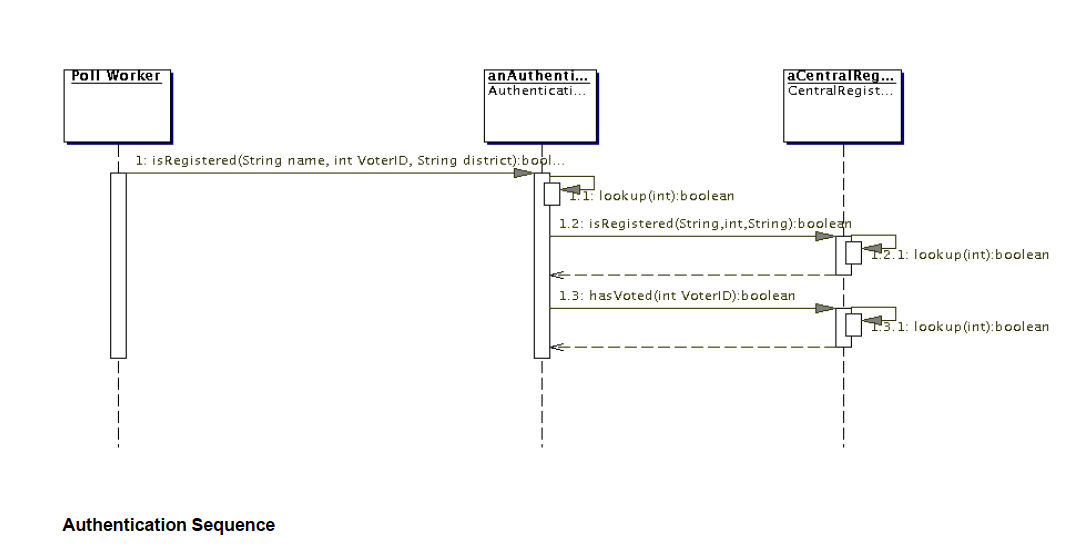
\includegraphics[width=1\textwidth]{Authentication.jpeg}
\caption{\label{fig:Auth}The diagram shows the sequence of operations that go behind Authenticating a user.}
\end{figure}

\subsection{Modifying VVPAT}
When a voter presses a button in the EVM, a paper slip is printed through the VVPAT. The slip contains the poll symbol and name of the candidate. It allows the voter to verify his/her choice.  After being visible to the voter from a glass case in the VVPAT for seven seconds, the ballot slip will be cut and dropped into the drop box in the VVPAT machine and a beep will be heard. VVPAT machines can be accessed by polling officers only. But to instill user confidence in the black box a paper trail will be put into a separate ballot box visible to the user. Apart from this, there are additional buttons on the VVPAT that allow a user to cancel the vote and recast it in case he/she finds an anomaly,

\begin{figure}
\centering
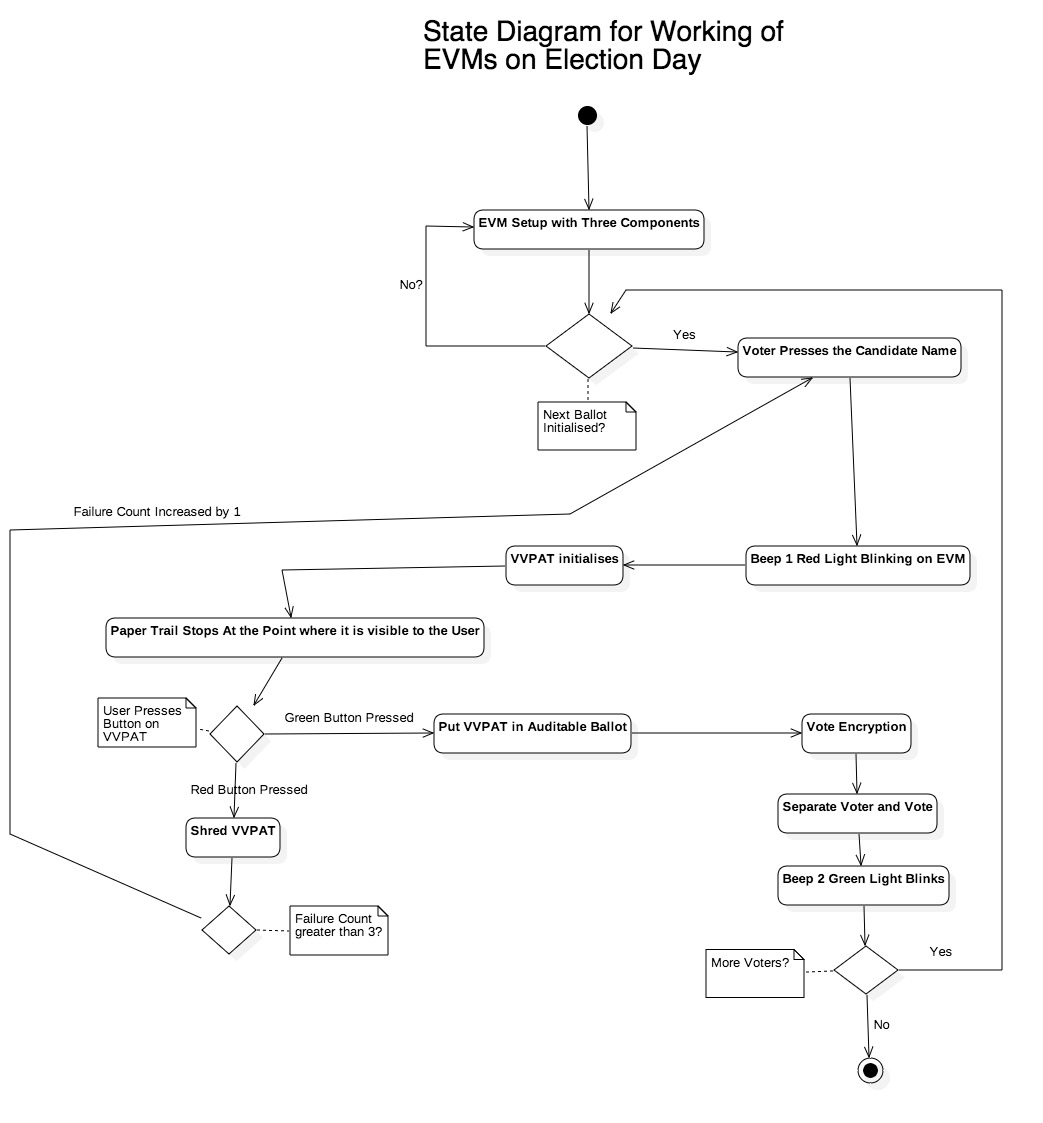
\includegraphics[width=1\textwidth]{EVM.jpg}
\caption{\label{fig:EVM}The diagram shows the various states  involved in the functioning of EVMs on election day.}
\end{figure}

\subsection{Self-Certifiable}
Any tampering to the machine must raise a red light on the machine that can not be undone. This ensures that the machine is not tampered with internally. Apart from this, an internal algorithm checker performs a Built in Self Test \textbf{(BIST)} to immediately output the present status of the machine. If the machine fails to succeed in the test, it must be immediately replaced.

\subsection{Impenetrable Hardware}
The hardware for the EVM will be impenetrable. The resent system has a lot of removable parts. The EVMs thus designed will  be compact and only one removable memory access slot, that can not be opened without the two level finger-print authentication of nodal officers at the booth and district level.
The system will not offer any options of tampering with the hardware and thus we would only need to work over the software integrity.

\subsection{Self-Identification}
This is an important feature that will ensure that the EVMs are not replaced on the polling site. The EVMs will contain a unique metal strip with encoded Machine Address, apart from a Hologram of the ECI that will be a certificate of the machine being the original one.

\subsection{Unique Encryption Scheme}
We will be utilizing the fingerprint of each and every individual to create a unique encryption algorithm that can only be accessed by the authorities at the EIC.

We decide to encrypt the data again because votes can come from many different pollsites, which may have different secret keys. Even same poll sites can have different session keys at different times. So to remove the complexity of storing the keys , we can uniformly encrypt the data.

One other reason is that now we can afford (time-wise) to use PKI, so that the
machine can only encrypt the data and decryption can take place after an human intervention.

\section{Discussion and Conclusion}
In spite of the potential advantages e-voting might bring to the polling station, such as improved turn out, accessibility for impaired people, and improved accuracy and speed, its adoption in various countries has been slow and/or the cause of great debates and controversies.

Another option is \textbf{precinct-count optical scan (PCOS)} voting, where voters fill out paper ballots that are scanned by a voting machine at the polling station before being placed in a ballot box. Attacking either of these systems would require tampering with both the paper records and the electronic records, provided that routine audits are performed to make sure these redundant sets of records agree. A third
option is to return to simple paper ballots. Despite all of their known weaknesses, simple paper ballots provide a \textbf{high degree of transparency}, so fraud that does occur will be more likely to be detected.

\section{References}
\begin{enumerate}
\item Formal Specification and Analysis of an e-Voting System by Komminist Weldemariam, Richard A. Kemmerer and Adolfo Villafiorita.
\item Security Analysis of India’s Electronic Voting Machines by Scott Wolchok, Hari K. Prasad and Rop Gonggrijp.
\item \href{http://eci.nic.in/eci/eci.html}{Election Commission of India}
\item \href{http://eci.nic.in/eci_main1/current/ChallengeEVM20052017.pdf}{EVM Challenge: ECI}
\item \href{https://www.huffingtonpost.in/ankit-lal/dear-election-commission-here-s-why-your-evm-hackathon-is-a-j_a_22108571/}{Huffington Post: On the EVM Challenge}
\item \href{https://www.ndtv.com/india-news/election-commission-evm-challenge-today-aap-hackathon-too-10-points-1707370}{NDTV: EVM Hackathon's that weren't}
\item \href{https://indiaevm.org}{Vulnerability of the Indian EVM}
\item \href{http://eci.nic.in/eci_main1/evm.aspx}{FAQs on EVM by ECI}
\item \href{http://eci.nic.in/eci_main1/evm1.aspx}{Demonstartion of Working of EVMs by ECI}
\item \href{https://www.iitbhilai.ac.in/index.php?pid=admin_messagefromdirector}{Information on Rajat Moona}
\item \href{https://blogs.timesofindia.indiatimes.com/toi-edit-page/evms-do-stellar-service-as-messengers-of-the-peoples-mandate-and-every-winning-candidate-loves-them/}{Rajat Moona on the credibility of EVMs: TOI}
\item \href{https://en.wikipedia.org/wiki/Electronic_voting_by_country}{Electronic Voting Status in Various Countries}
\item Functional Requirements for a Secure Electronic Voting System by Costas Ambrinoudakis and Spyros Kokolakis.
\item Designing a Voting Machine for Testing and Verification by Cynthia Sturton
\end{enumerate}


\end{document}